\documentclass[border=2pt]{standalone}
\usepackage{tikz}
\usetikzlibrary{arrows.meta,chains,%
                    decorations.pathreplacing}
\usetikzlibrary{matrix,positioning,arrows.meta,arrows}
\usetikzlibrary{calc}
\usepackage{multirow,array}

\newcommand\hlight[1]{\tikz[overlay, remember picture]\node[rectangle,fill=blue!50,rounded corners,fill opacity = 0.2,draw,thick,text opacity =1] {$#1$};} 

\newcommand\diag[4]{%
%  \multicolumn{1}{p{#2}|}
  \parbox[t]{#2}%
  {\hskip-\tabcolsep
  $\vcenter{\begin{tikzpicture}[baseline=0,anchor=south west,inner sep=#1]
  \path[use as bounding box] (0,0) rectangle (\baselineskip,\baselineskip);
  \node[minimum width={#2+1\tabcolsep},minimum height=\baselineskip+\extrarowheight] (box) {};
%  \draw (box.north west) -- (box.south east);
  \node[anchor=south west] at (box.south) {#3};
  \node[anchor=north east] at (box.east) {#4};
 \end{tikzpicture}}$\hskip-\tabcolsep}}

\tikzset{
mymat/.style={
  matrix of nodes,
  nodes in empty cells,
  text height=2.5ex,
  text depth=0.75ex,
  text width=3.25ex,
  align=center,
  column sep=-\pgflinewidth
  },
cartesian/.style={
  align=center, inner sep=1pt, text centered,
  font=\sffamily, circle, black, draw=black, 
  fill=white, text=black, minimum width=0.5em, minimum height=1em
  }
}
\tikzset{
  rows/.style 2 args={
    sub@rows/.style={row ##1 column #2/.style={nodes={rectangle,draw=black}}},
    sub@rows/.list={#1}
  },
  box/.style 2 args={
    sub@box/.style={rows={#1}{##1}},
    sub@box/.list={#2}
  }
}
\begin{document}

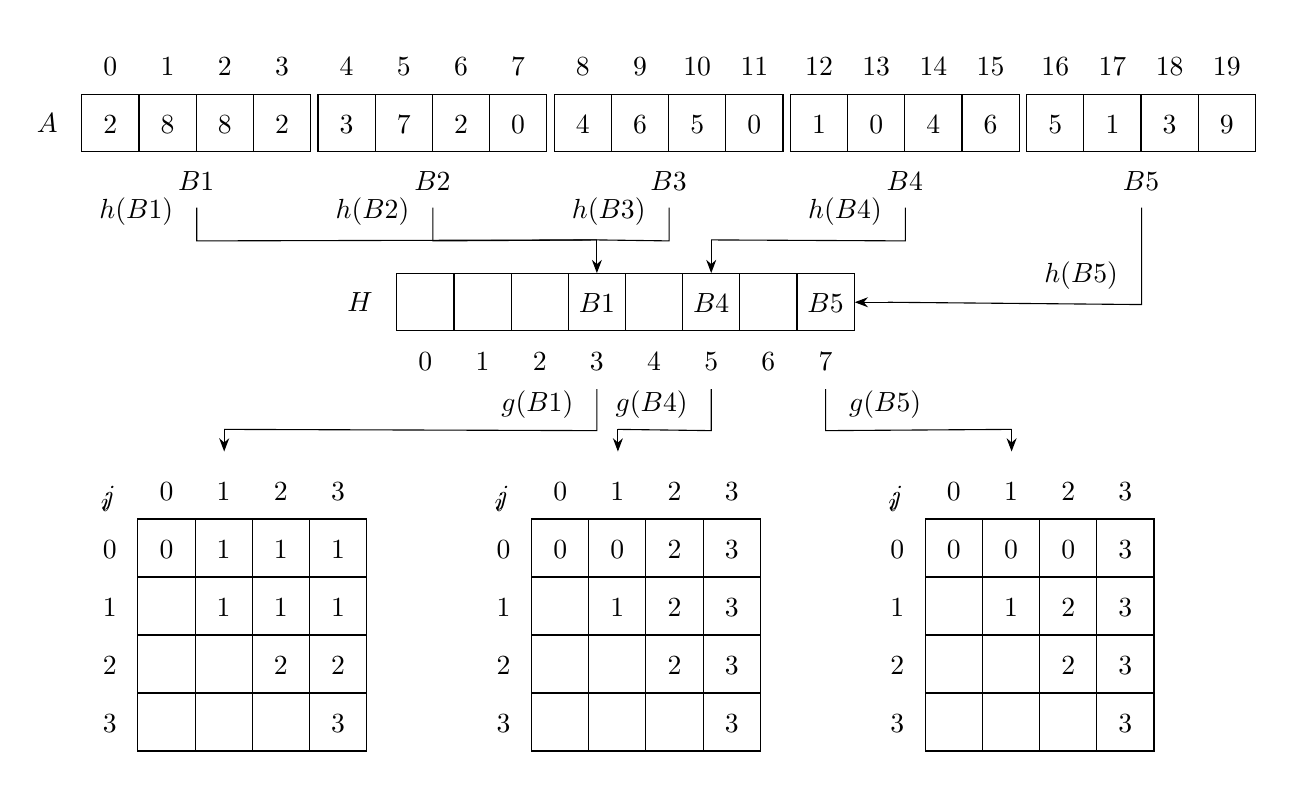
\begin{tikzpicture}[>=latex]
\matrix[mymat,anchor=west,
    box={2}{1, 2, 3, 4}]
at (0,0) 
(mat1)
{ 
  0 & 1 & 2 & 3 \\
  2 & 8 & 8 & 2 \\ };
\matrix[mymat,anchor=west,
    box={2}{1, 2, 3, 4}]
at (3,0) 
(mat2)
{ 4 & 5 & 6 & 7 \\
  3 & 7 & 2 & 0 \\ };
\matrix[mymat,anchor=west,
    box={2}{1, 2, 3, 4}]
at (6,0) 
(mat3)
{ 8 & 9 & 10 & 11 \\
  4 & 6 & 5 & 0 \\ };
\matrix[mymat,anchor=west,
    box={2}{1, 2, 3, 4}]
at (9,0) 
(mat4)
{ 
  12 & 13 & 14 & 15 \\
  1 & 0 & 4 & 6 \\ };
\matrix[mymat,anchor=west,
    box={2}{1, 2, 3, 4}]
at (12,0) 
(mat5)
{ 16 & 17 & 18 & 19 \\
  5 & 1 & 3 & 9 \\ };

\node[below=0pt of mat1]{$B1$};
\node[below=0pt of mat2]{$B2$};
\node[below=0pt of mat3]{$B3$};
\node[below=0pt of mat4]{$B4$};
\node[below=0pt of mat5]{$B5$};

\matrix[mymat,anchor=west,
    box={1}{1, 2, 3, 4, 5, 6, 7, 8}]
at (4,-3) 
(matH)
{   &   &   & $B1$ &   & $B4$ & & $B5$ \\
  0 & 1 & 2 & 3 & 4 & 5 & 6 & 7\\ };

\node[left=5pt of mat1-2-1.west]{$A$ \\};
\node[left=5pt of matH-1-1.west]{$H$ \\};



\begin{scope}
\coordinate(B1) at([yshift=-20pt]mat1-2-2.south east);
\coordinate(B1f) at([yshift=-32pt]mat1-2-2.south east);
\coordinate(B2) at([yshift=-20pt]mat2-2-2.south east);
\coordinate(B2f) at([yshift=-32pt]mat2-2-2.south east);
\coordinate(B3) at([yshift=-20pt]mat3-2-2.south east);
\coordinate(B3f) at([yshift=-32pt]mat3-2-2.south east);

\node[above left=2pt and 5pt of B1f] {$h(B1)$\\};
\node[above left=2pt and 5pt of B2f] {$h(B2)$\\};
\node[above left=2pt and 5pt of B3f] {$h(B3)$\\};

\coordinate(type1f) at([yshift=12pt]matH-1-4.north);
\draw (B1) -- (B1f) -- (type1f);
\draw (B2) -- (B2f) -- (type1f);
\draw (B3) -- (B3f) -- (type1f);
\draw[-{Stealth[scale=1]}] (type1f) -- (matH-1-4.north);

\end{scope}

\begin{scope}
\coordinate(B4) at([yshift=-20pt]mat4-2-2.south east);
\coordinate(B4f) at([yshift=-32pt]mat4-2-2.south east);

\node[above left=2pt and 5pt of B4f] {$h(B4)$\\};

\coordinate(type2f) at([yshift=12pt]matH-1-6.north);
\draw (B4) -- (B4f) -- (type2f);
\draw[-{Stealth[scale=1]}] (type2f) -- (matH-1-6.north);
\end{scope}

\begin{scope}
\coordinate(B5) at([yshift=-20pt]mat5-2-2.south east);
\coordinate(B5f) at([yshift=-55pt]mat5-2-2.south east);

\node[above left=2pt and 5pt of B5f] {$h(B5)$\\};

\coordinate(type3f) at([xshift=12pt]matH-1-8.east);
\draw (B5) -- (B5f) -- (type3f);
\draw[-{Stealth[scale=1]}] (type3f) -- (matH-1-8.east);
\end{scope}

% type of a Cartesian tree

\matrix[mymat,anchor=west,
    box={2,3,4, 5}{2, 3, 4, 5}]
at (0,-6.5) 
(type1)
{ 
  \diag{.0em}{0.0em}{$j$}{$i$} & 0 & 1 & 2 & 3 \\
  0 & 0 & 1 & 1 & 1 \\ 
  1 &   & 1 & 1 & 1 \\ 
  2 &   &   & 2 & 2 \\
  3 &   &   &   & 3 \\};

\matrix[mymat,anchor=west,
    box={2,3,4, 5}{2, 3, 4, 5}]
at (5,-6.5) 
(type2)
{ 
  \diag{.0em}{0.0em}{$j$}{$i$} & 0 & 1 & 2 & 3 \\
  0 & 0 & 0 & 2 & 3 \\ 
  1 &   & 1 & 2 & 3 \\ 
  2 &   &   & 2 & 3 \\
  3 &   &   &   & 3 \\};

\matrix[mymat,anchor=west,
    box={2,3,4, 5}{2, 3, 4, 5}]
at (10,-6.5) 
(type3)
{ 
  \diag{.0em}{0.0em}{$j$}{$i$} & 0 & 1 & 2 & 3 \\
  0 & 0 & 0 & 0 & 3 \\ 
  1 &   & 1 & 2 & 3 \\ 
  2 &   &   & 2 & 3 \\
  3 &   &   &   & 3 \\};

% link to table

\begin{scope}
\coordinate(Htype1) at([yshift=0pt]matH-2-4.south);
\coordinate(Htype1f) at([yshift=-15pt]matH-2-4.south);

\node[above left=1pt and 5pt of Htype1f] {$g(B1)$\\};

\coordinate(type1f) at([yshift=8pt]type1.north);
\draw (Htype1) -- (Htype1f) -- (type1f);
\draw[-{Stealth[scale=1]}] (type1f) -- (type1.north);
\end{scope}

\begin{scope}
\coordinate(Htype2) at([yshift=0pt]matH-2-6.south);
\coordinate(Htype2f) at([yshift=-15pt]matH-2-6.south);

\node[above left=1pt and 5pt of Htype2f] {$g(B4)$\\};

\coordinate(type2f) at([yshift=8pt]type2.north);
\draw (Htype2) -- (Htype2f) -- (type2f);
\draw[-{Stealth[scale=1]}] (type2f) -- (type2.north);
\end{scope}

\begin{scope}
\coordinate(Htype3) at([yshift=0pt]matH-2-8.south);
\coordinate(Htype3f) at([yshift=-15pt]matH-2-8.south);

\node[above right=1pt and 5pt of Htype3f] {$g(B5)$\\};

\coordinate(type3f) at([yshift=8pt]type3.north);
\draw (Htype3) -- (Htype3f) -- (type3f);
\draw[-{Stealth[scale=1]}] (type3f) -- (type3.north);
\end{scope}

\end{tikzpicture}

\end{document}